\documentclass[a4paper,11pt]{article}
\usepackage[top = 2.5cm, bottom = 2.5cm, left = 2.5cm, right = 2.5cm]{geometry} 
\usepackage[spanish]{babel} %Castellanización
\usepackage[T1]{fontenc}
\usepackage[utf8]{inputenc}
\usepackage{amssymb, amsmath}
\usepackage{multirow}
\usepackage{booktabs}
\usepackage{graphicx}
\usepackage{setspace}
\setlength{\parindent}{0.25in}
\usepackage{float}
\usepackage{fancyhdr}
\usepackage[usenames]{color}
%\documentclass[tikz, border=2mm]{standalone}
\usepackage{karnaugh-map}
\usepackage{graphicx,caption}
\usepackage{verbatim}
\usepackage{hyperref}
\usepackage{algorithmic}
\usepackage{algorithm}
\usepackage{float}
\pagestyle{fancy}
\fancyhf{}

\lhead{\footnotesize INF256: Laboratorio 1}%
\rhead{\footnotesize CS JS - P200/201}
\cfoot{\footnotesize \thepage} 

\begin{document}


%%%%%%%%%%%%%%%%%%%%%%%%%%%%%%%%%%%%%%%%%%%%%%%%
%%%%%%%%%%%%%%%%%%%%%%%%%%%%%%%%%%%%%%%%%%%%%%%%

\thispagestyle{empty} % This command disables the header on the first page. 

  \begin{minipage}{.2\linewidth}
    \begin{flushleft}
      
\includegraphics[height = 1.5cm]{Imagenes/UTFSM.jpg}
    \end{flushleft}
  \end{minipage}
  \hfill
  \begin{minipage}{.7\linewidth}
    \begin{flushright}
        Universidad Técnica Federico Santa María \\
        Departamento de Informática\\
        INF256 - Redes de Computadores\\
    \end{flushright}
  \end{minipage}
%\begin{center}
%    \hrule
%\end{center}

\vfill % Now we want to add some vertical space in between the line and our title.
\begin{center}
	{\Large Laboratorio 1\\}
	{\huge Tic Tac Toe\\}
	\vspace{.5cm}
	\hrule
	\vspace{.5cm}
        % YOUR NAMES GO HERE
    {\large Catalina Sierra H.} - catalina.sierrah@usm.cl - Rol 201973557-8\\
	{\large José Southerland S.} - jose.southerland@usm.cl - Rol 201973526-8\\
	
\end{center}
\vfill
\newpage
\tableofcontents
\newpage
\section{Preguntas y respuestas}
\begin{enumerate}
    \item Si se analiza el n\'umero de los mensajes enviados dentro de la aplicaci\'on. ¿C\'uantos son los que logra detectar Wireshark?. Y comparando en base al c\'odigo, ¿Es la misma cantidad?, si no lo es, ¿A qu\'e se deber\'a?
    \newline \textit{Respuesta}: En nuestro caso el n\'umero de mensajes enviados dentro de la aplicaci\'on depende del camino que tome el juego, es decir, si es que el bot no desea jugar solo se enviar\'ian 4 mensajes, tal como lo muestra el diagrama de la tarea. Pero si por ejemplo, estamos jugando y el bot quiso jugar en una casilla ocupada, servidor gato se cominicar\'a continuamente con el servidor intermediario y viceversa hasta encontrar una casilla vac\'ia.
    Wireshark en estos casos logra detectar todas las interacciones.
    
    \item ¿Cu\'a es el protocolo que se debiese ver a la hora de revisar el intercambio de mensajes en Wireshark? ¿Y cu\'ales encontr\'o?
    \newline \textit{Respuesta:} Se debiesen ver los protocolos UDP y TCP. En nuestro caso, además de dichos protocolos, se encontró el ICMP, que corresponde a Internet Control Message Protocol, y que aparece en la jugada ganadora, avisando que la dirección a la que se quiere llegar no es alcanzable.
    
    \item ¿El contenido de los mensajes dentro de Wireshark son legibles?, ¿Por qu\'e si? o  ¿Por qu\'e no?
    \newline \textit{Respuesta:} Los mensajes enviados dentro del juego no son legibles dentro de Wireshark, dado que dentro del código el envío de los mensajes vía UDP y TCP se encuentran codificados.
\end{enumerate}
 \newpage
\section{Anexo}

\begin{figure}[h]
    \centering
    {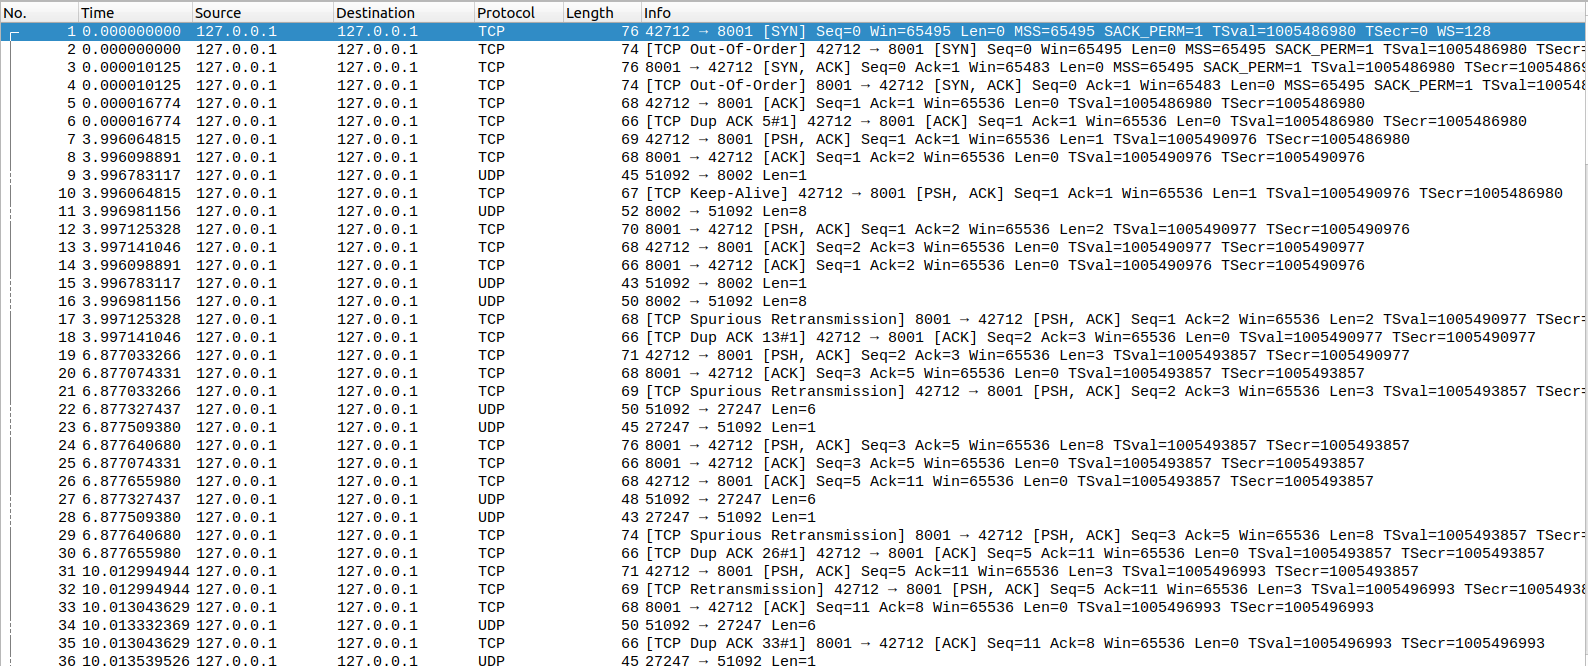
\includegraphics[width = 1.0\textwidth]{imagen-1.png}}
    \caption {Parte 1 juego de gato.}
\end{figure}

\begin{figure}[h]
    \centering
    {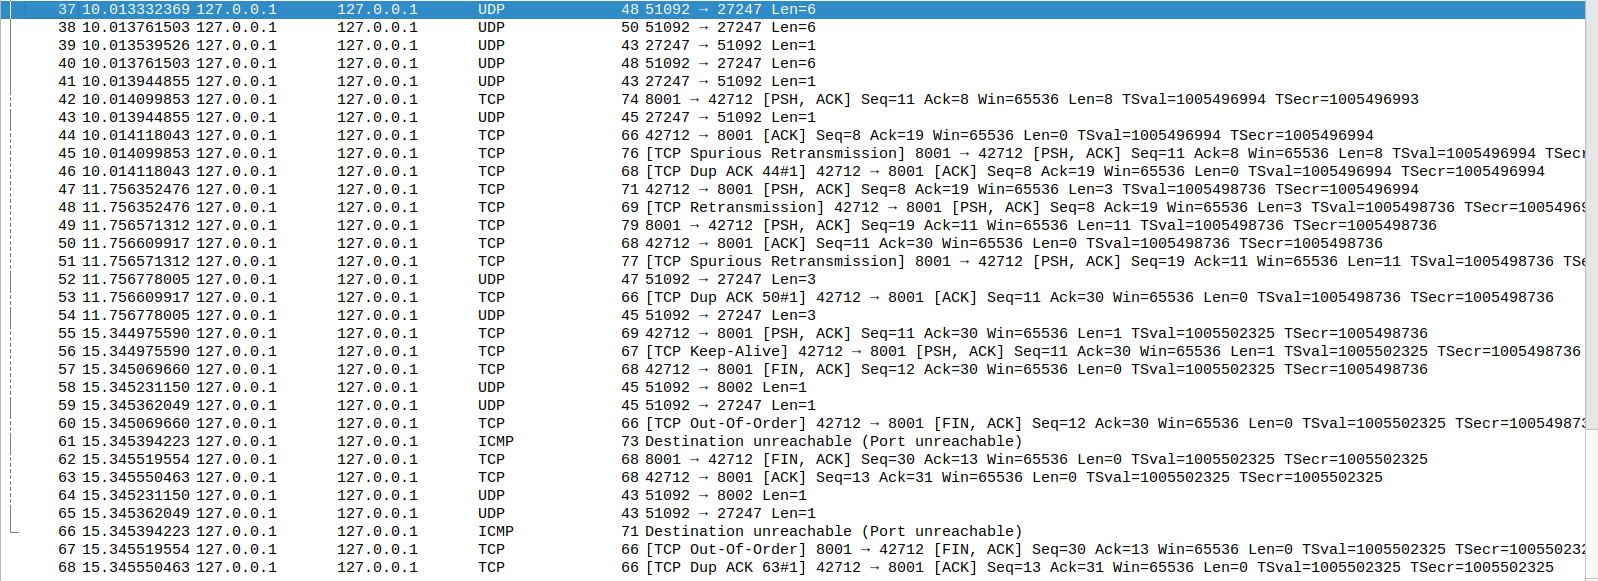
\includegraphics[width = 1.0\textwidth]{imagne-2.png}}
    \caption {Parte 2 juego de gato.}
\end{figure}

\begin{figure}[h]
    \centering
    {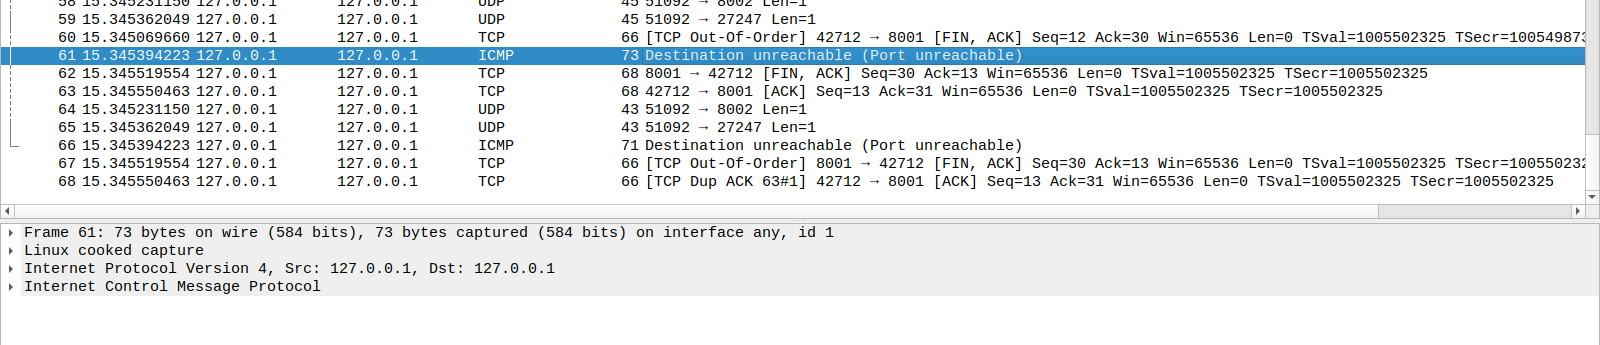
\includegraphics[width = 1.0\textwidth]{icmp.png}}
    \caption {Protocolo ICMP.}
\end{figure}

\begin{figure}[h]
    \centering
    {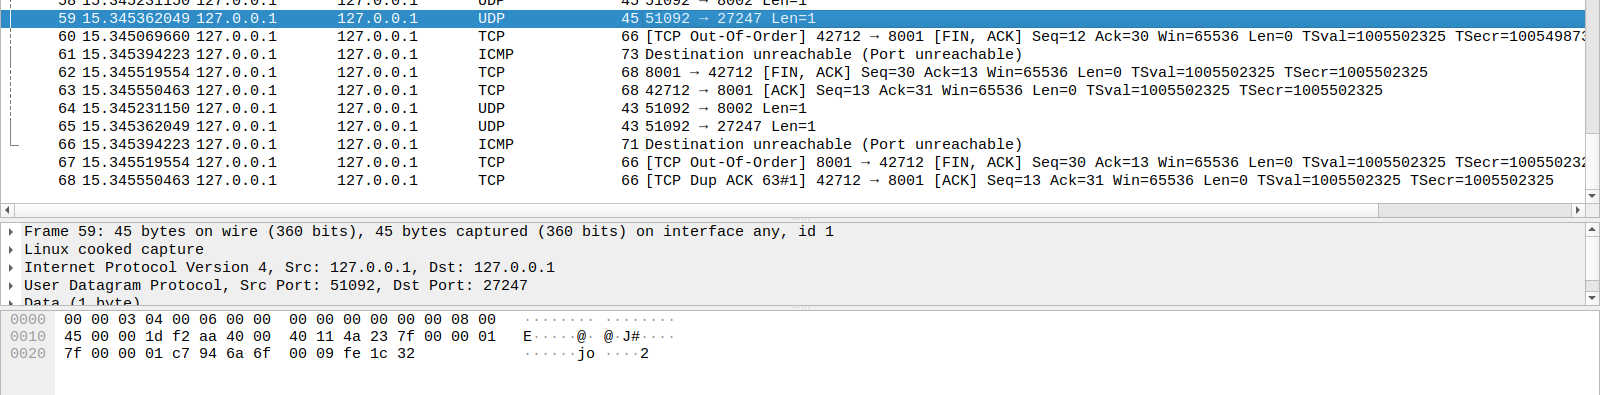
\includegraphics[width = 1.0\textwidth]{ilegible.png}}
    \caption {Mensajes ilegibles.}
\end{figure}

\vspace{.5cm}

\end{document}